\section{Implementation}
Realization of the design is covered in the implementation of the system.
The design is implemented in the Development stage.
Upon completion, the system is deployed to a \Ac{vps}, allowing for the service to be accessed on the internet.

\subsection{Android Application}
Figure \ref{fig:android_app_implementation} depicts the functionality and layout of the implemented android application.
Screenshots are taken of the application running in an Android emulator.

\begin{figure}[H]
\centering
    \subfigure[Idle state]
    {
        \centering
        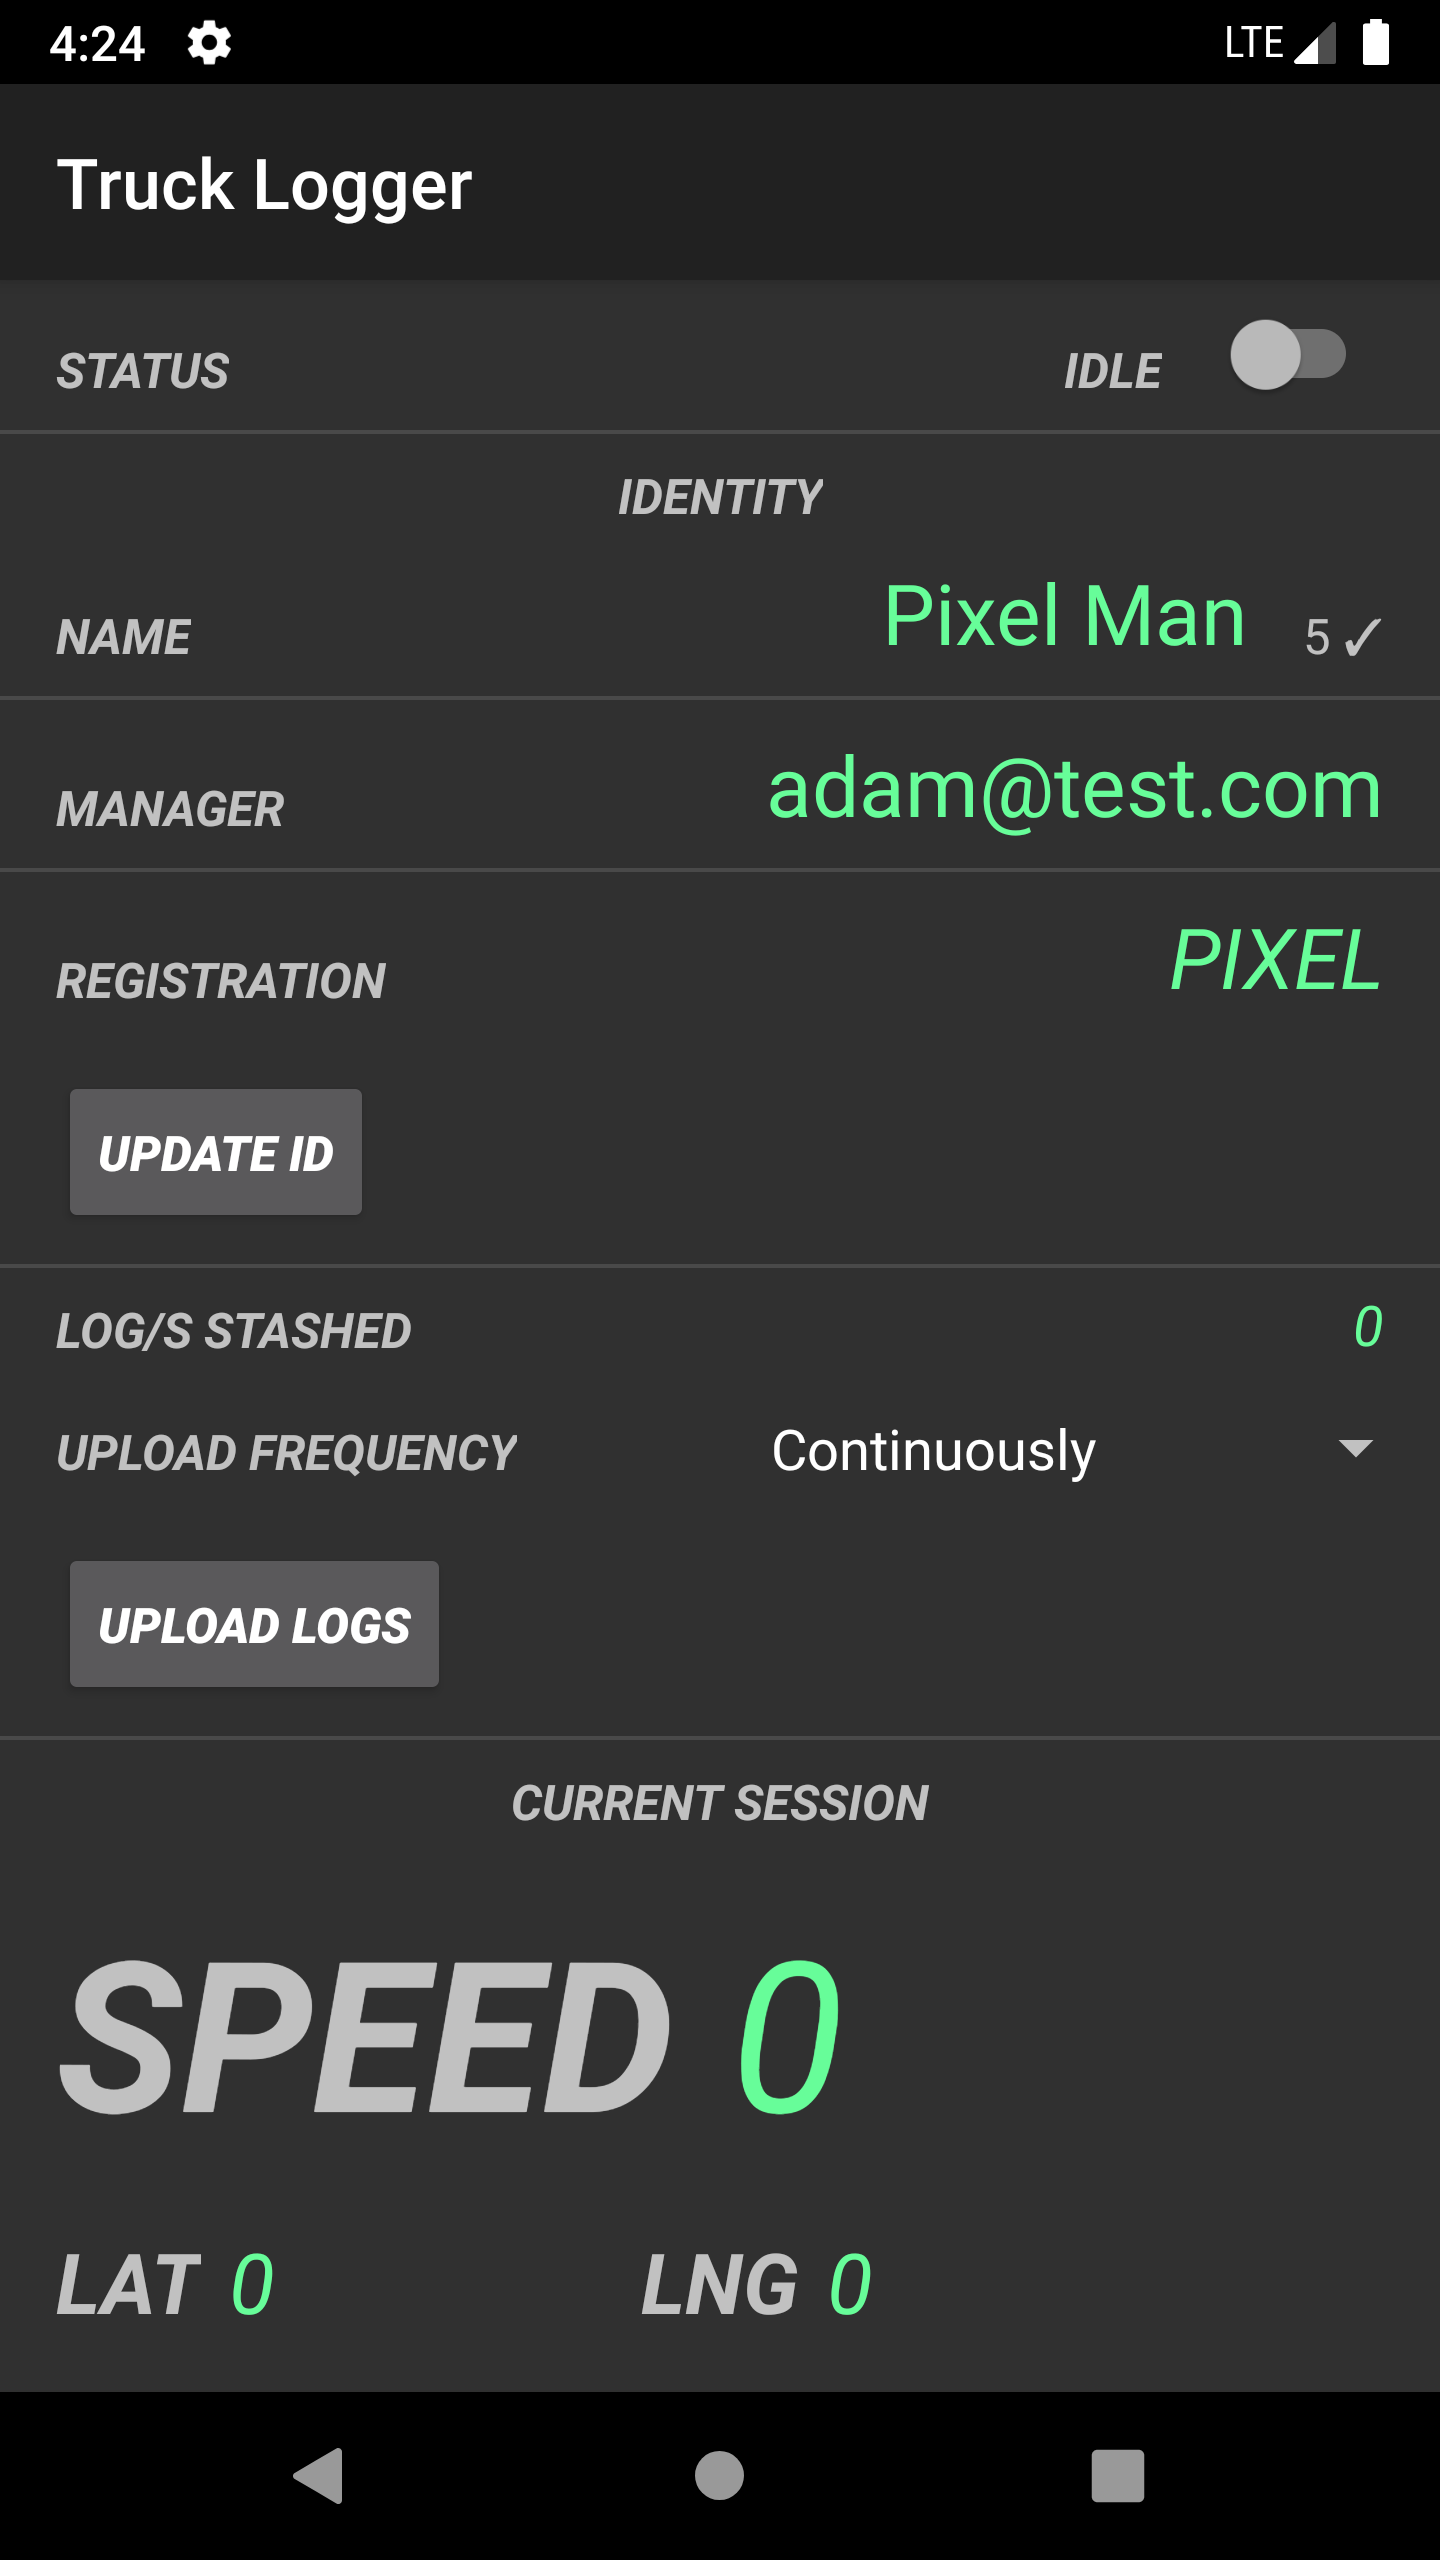
\includegraphics[height=2.5in]{android_app_idle.png}
        \label{fig:android_app_idle}
    }
    \subfigure[Running state]
    {
        \centering
        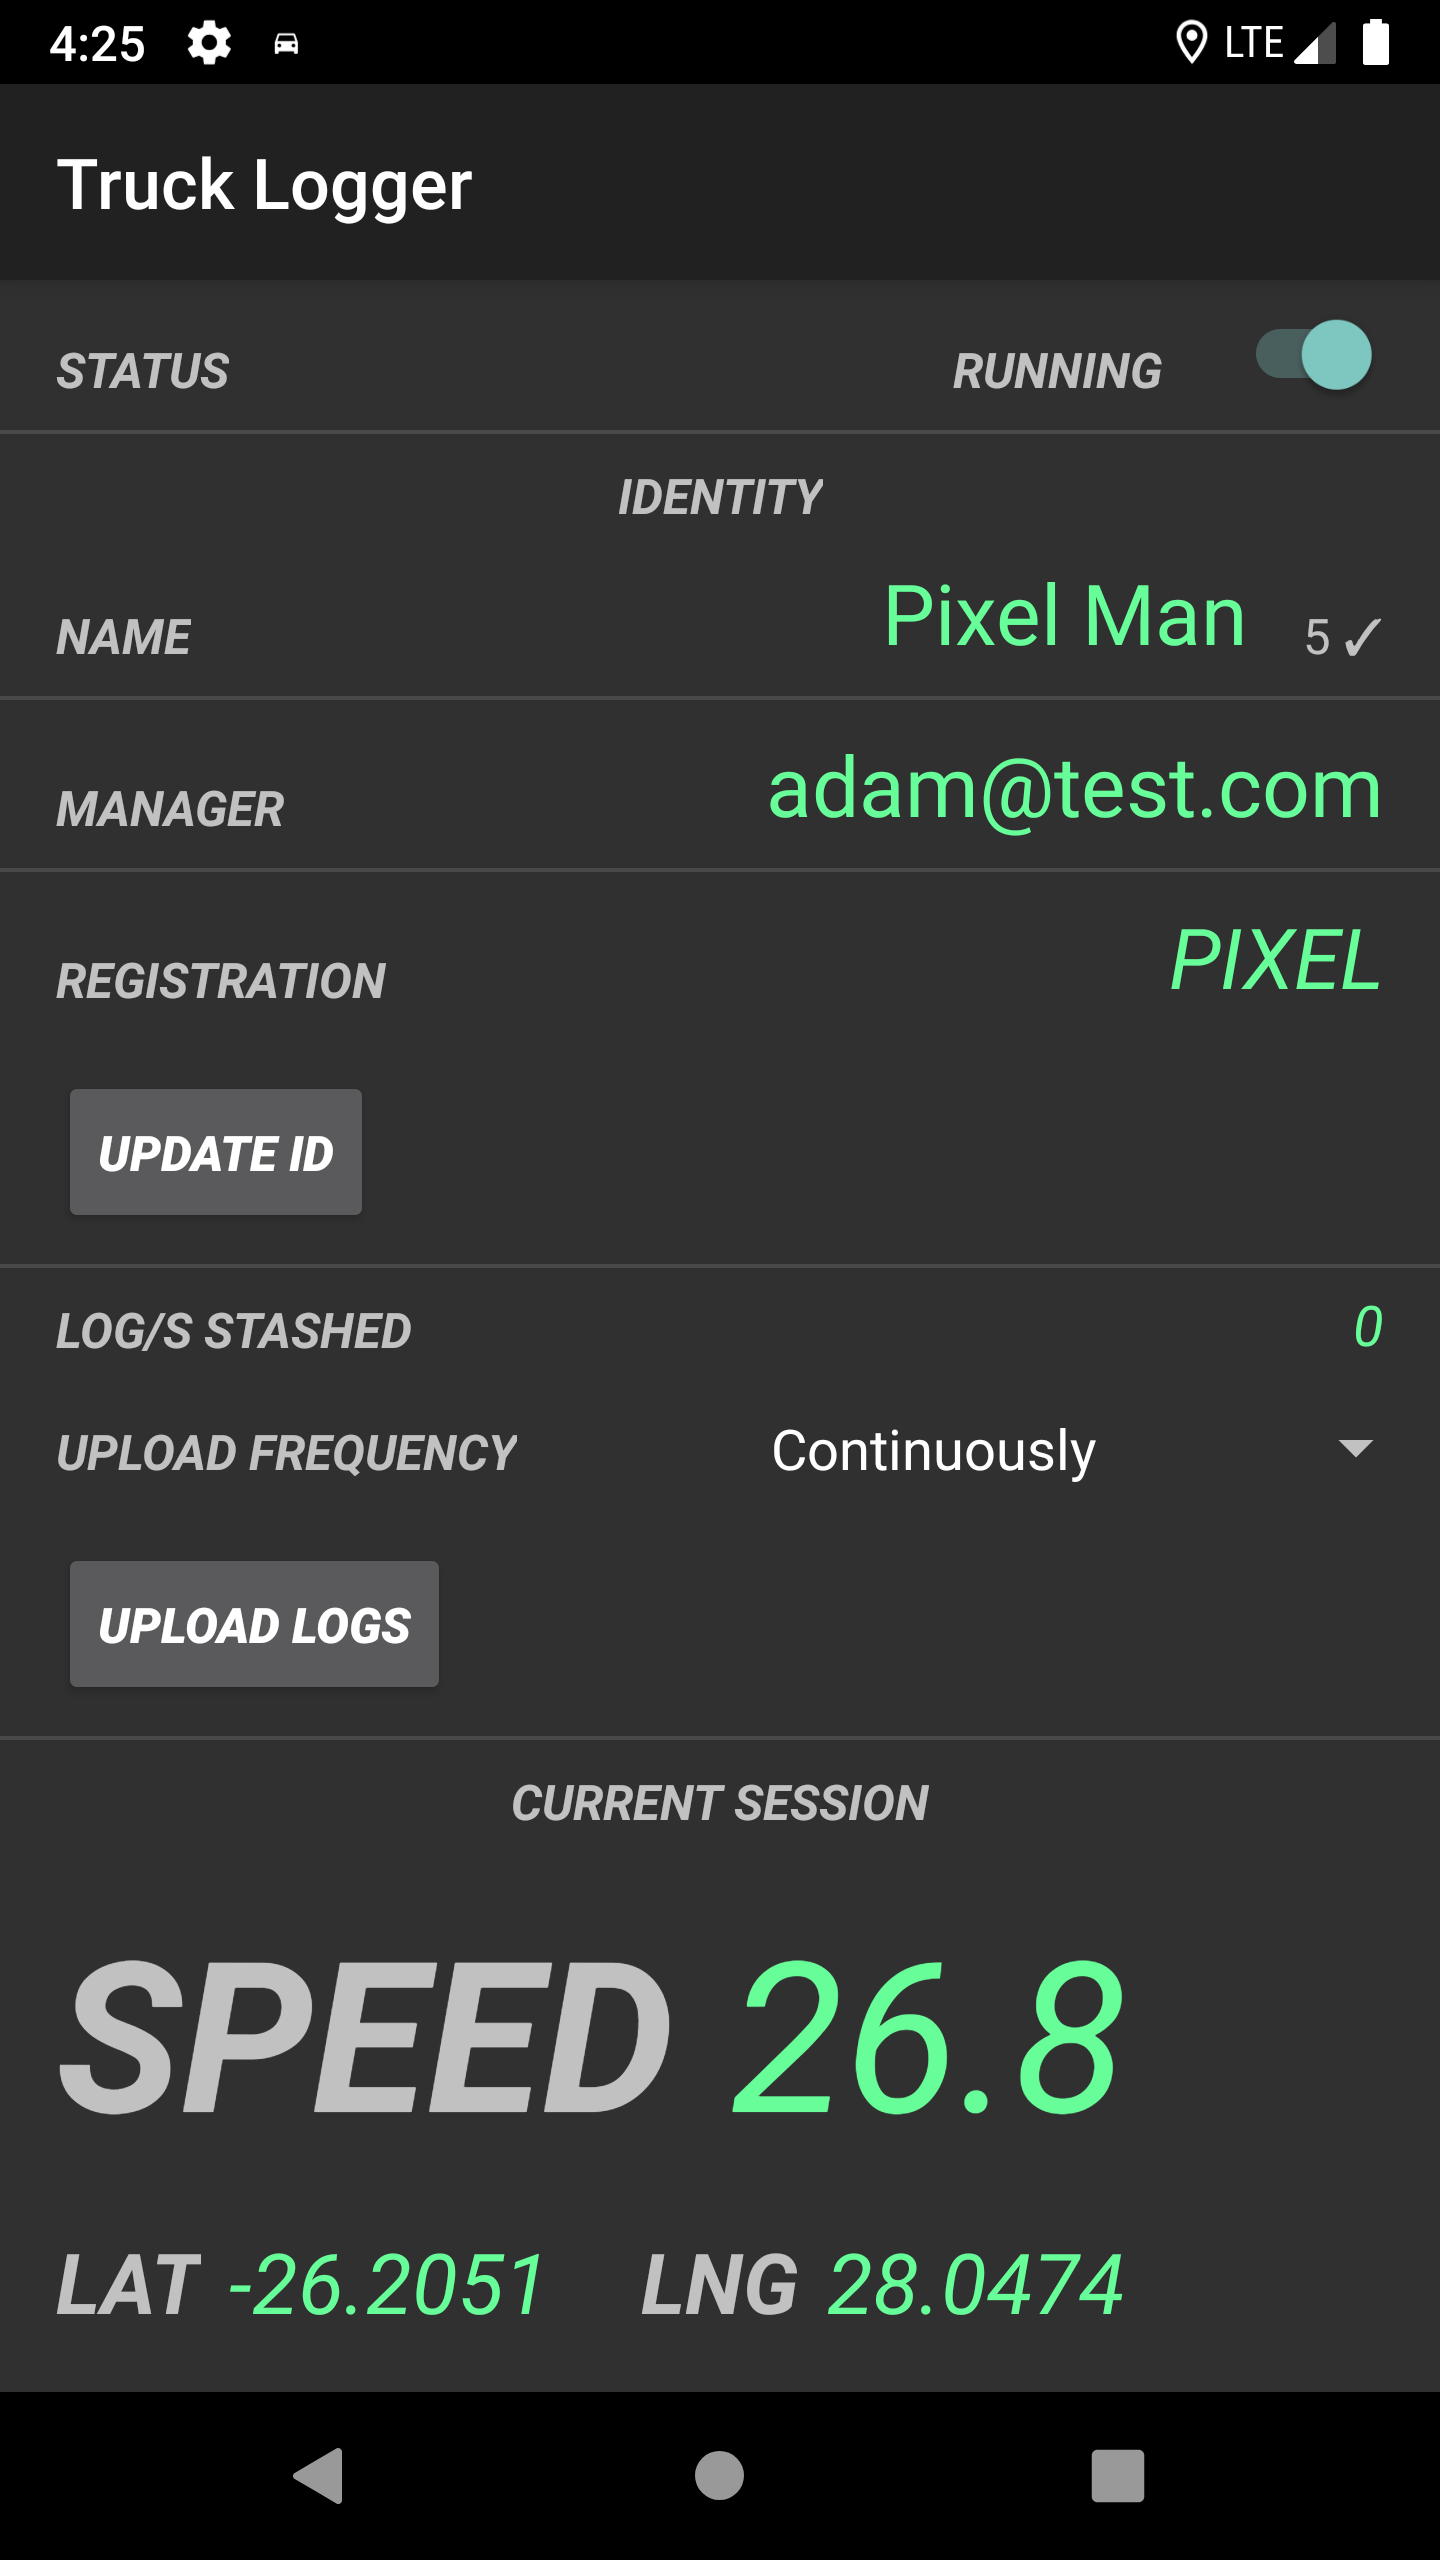
\includegraphics[height=2.5in]{android_app_running.png}
        \label{fig:android_app_running}
    }\\
    \subfigure[Background operation]
    {
        \centering
        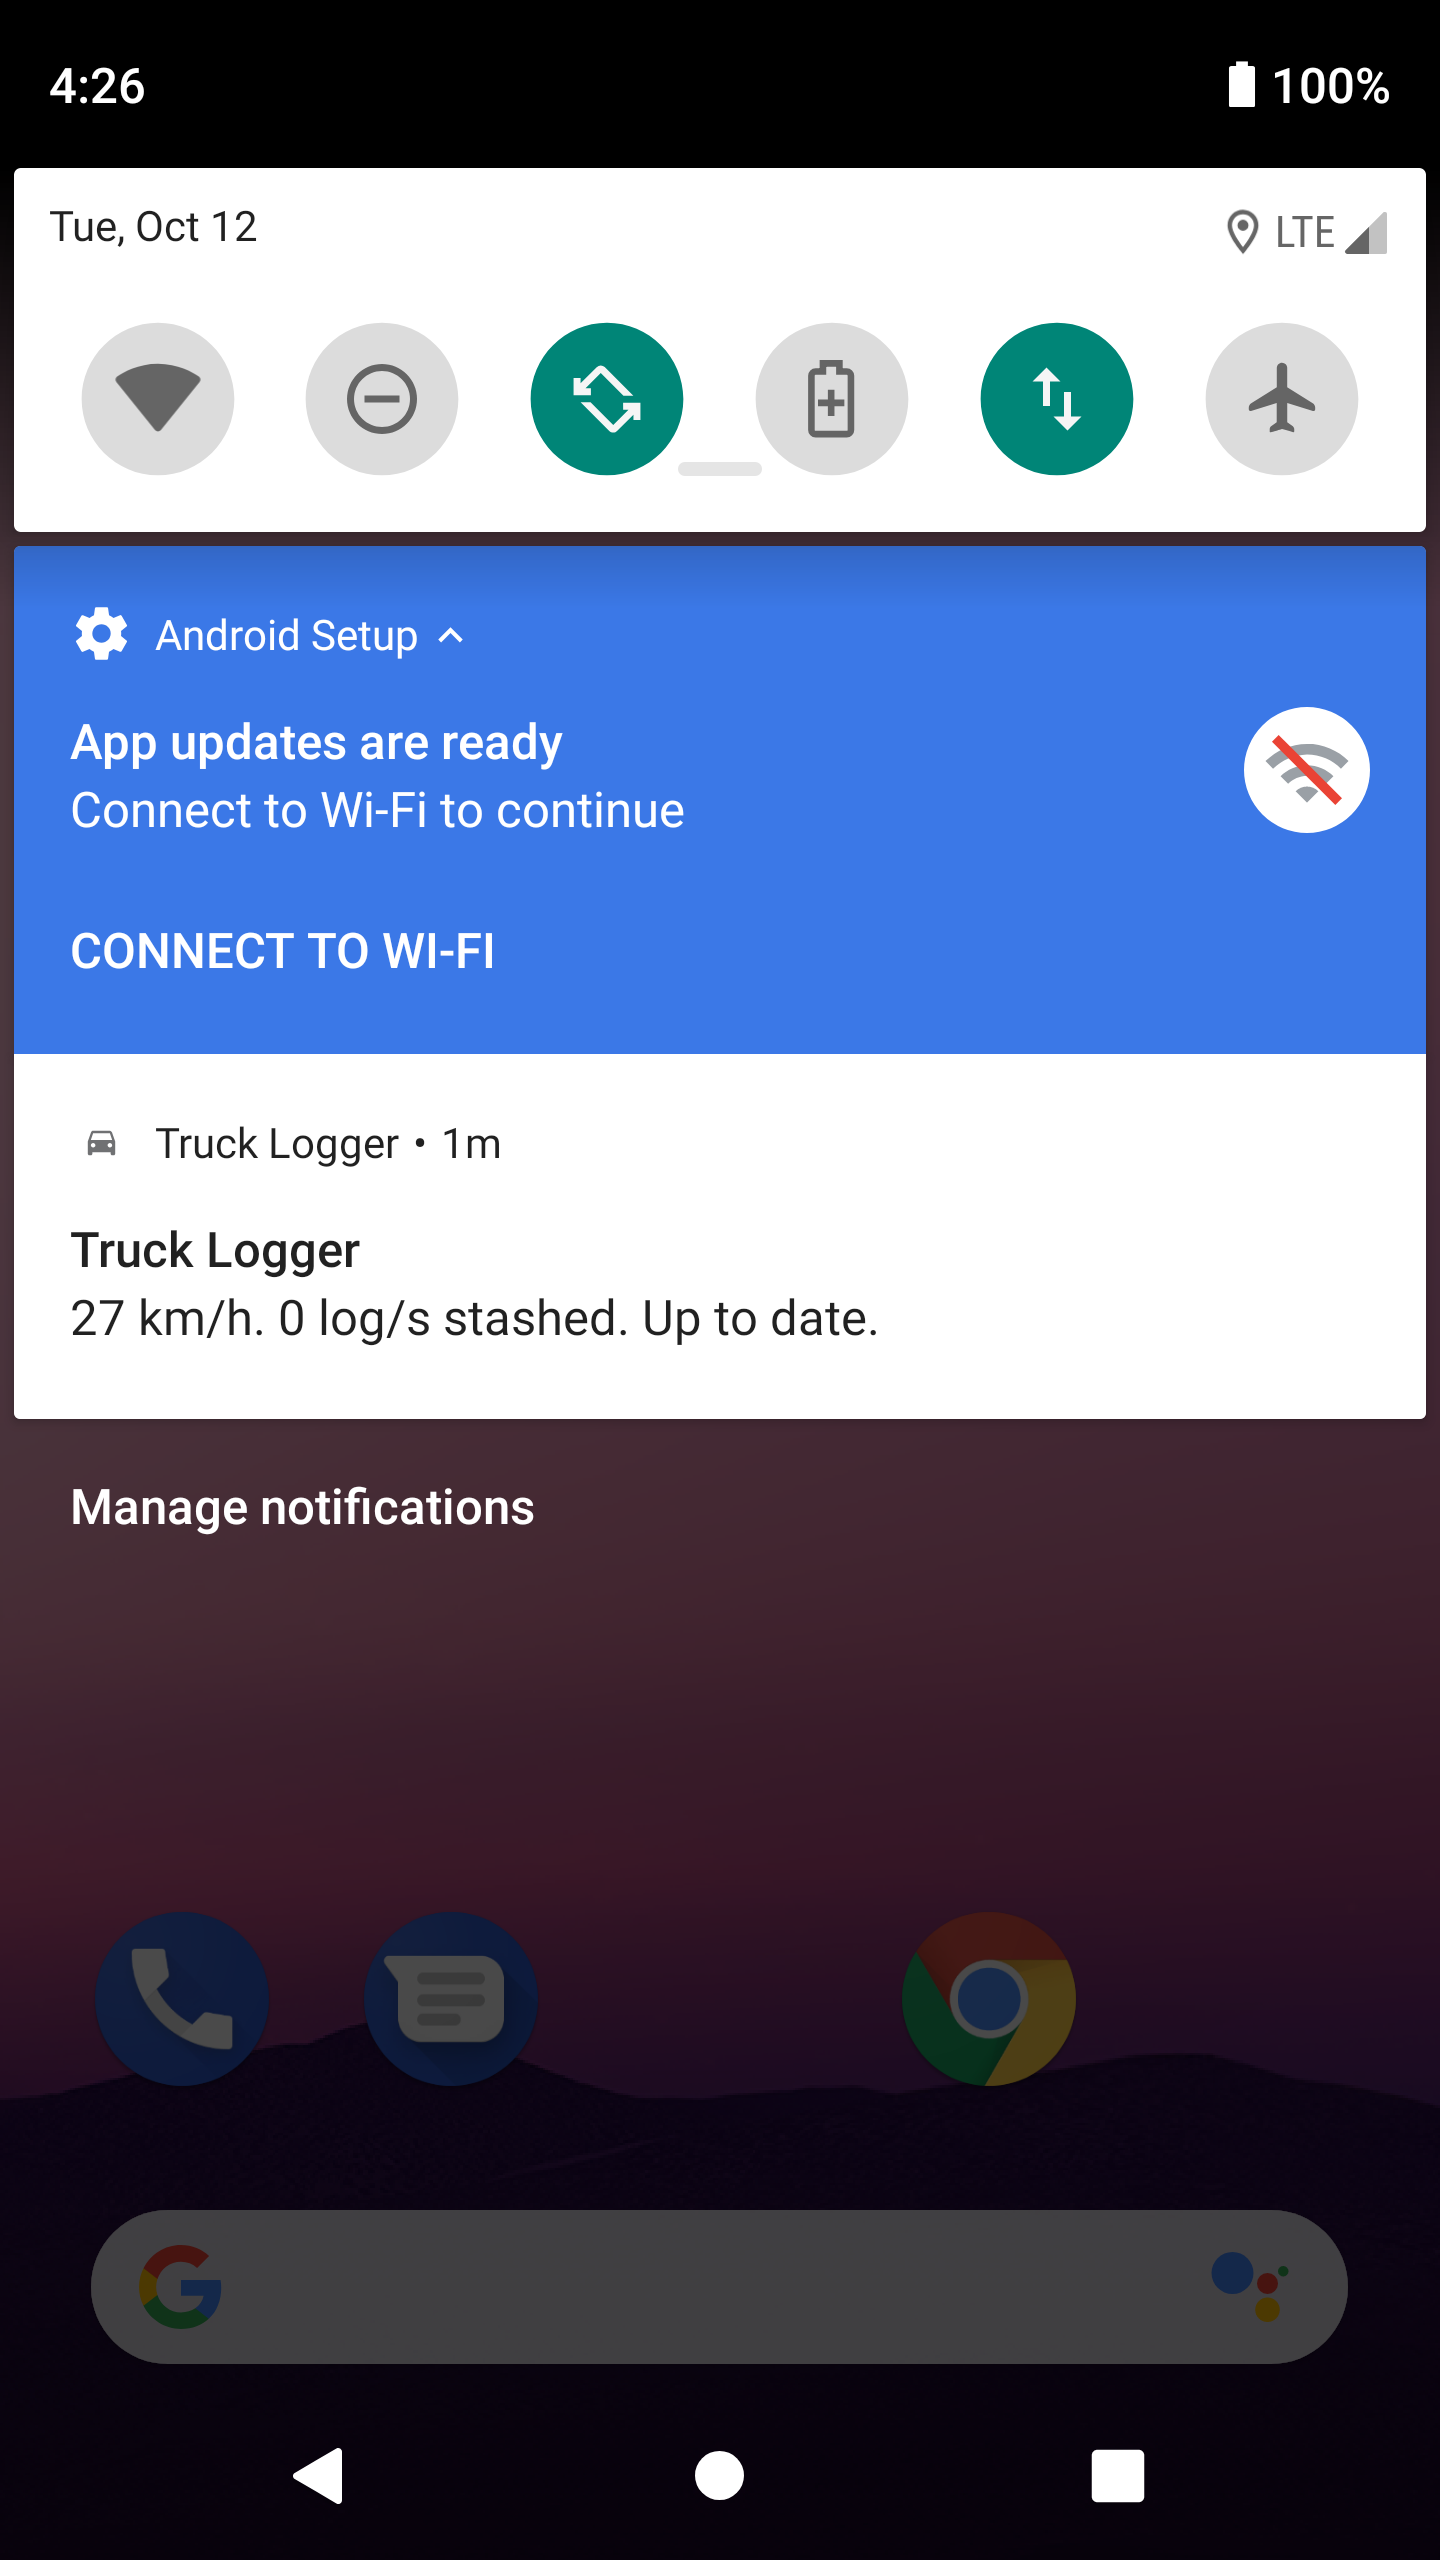
\includegraphics[height=2.5in]{android_app_background.png}
        \label{fig:android_app_background}
    }
    \subfigure[Stashing logs locally]
    {
        \centering
        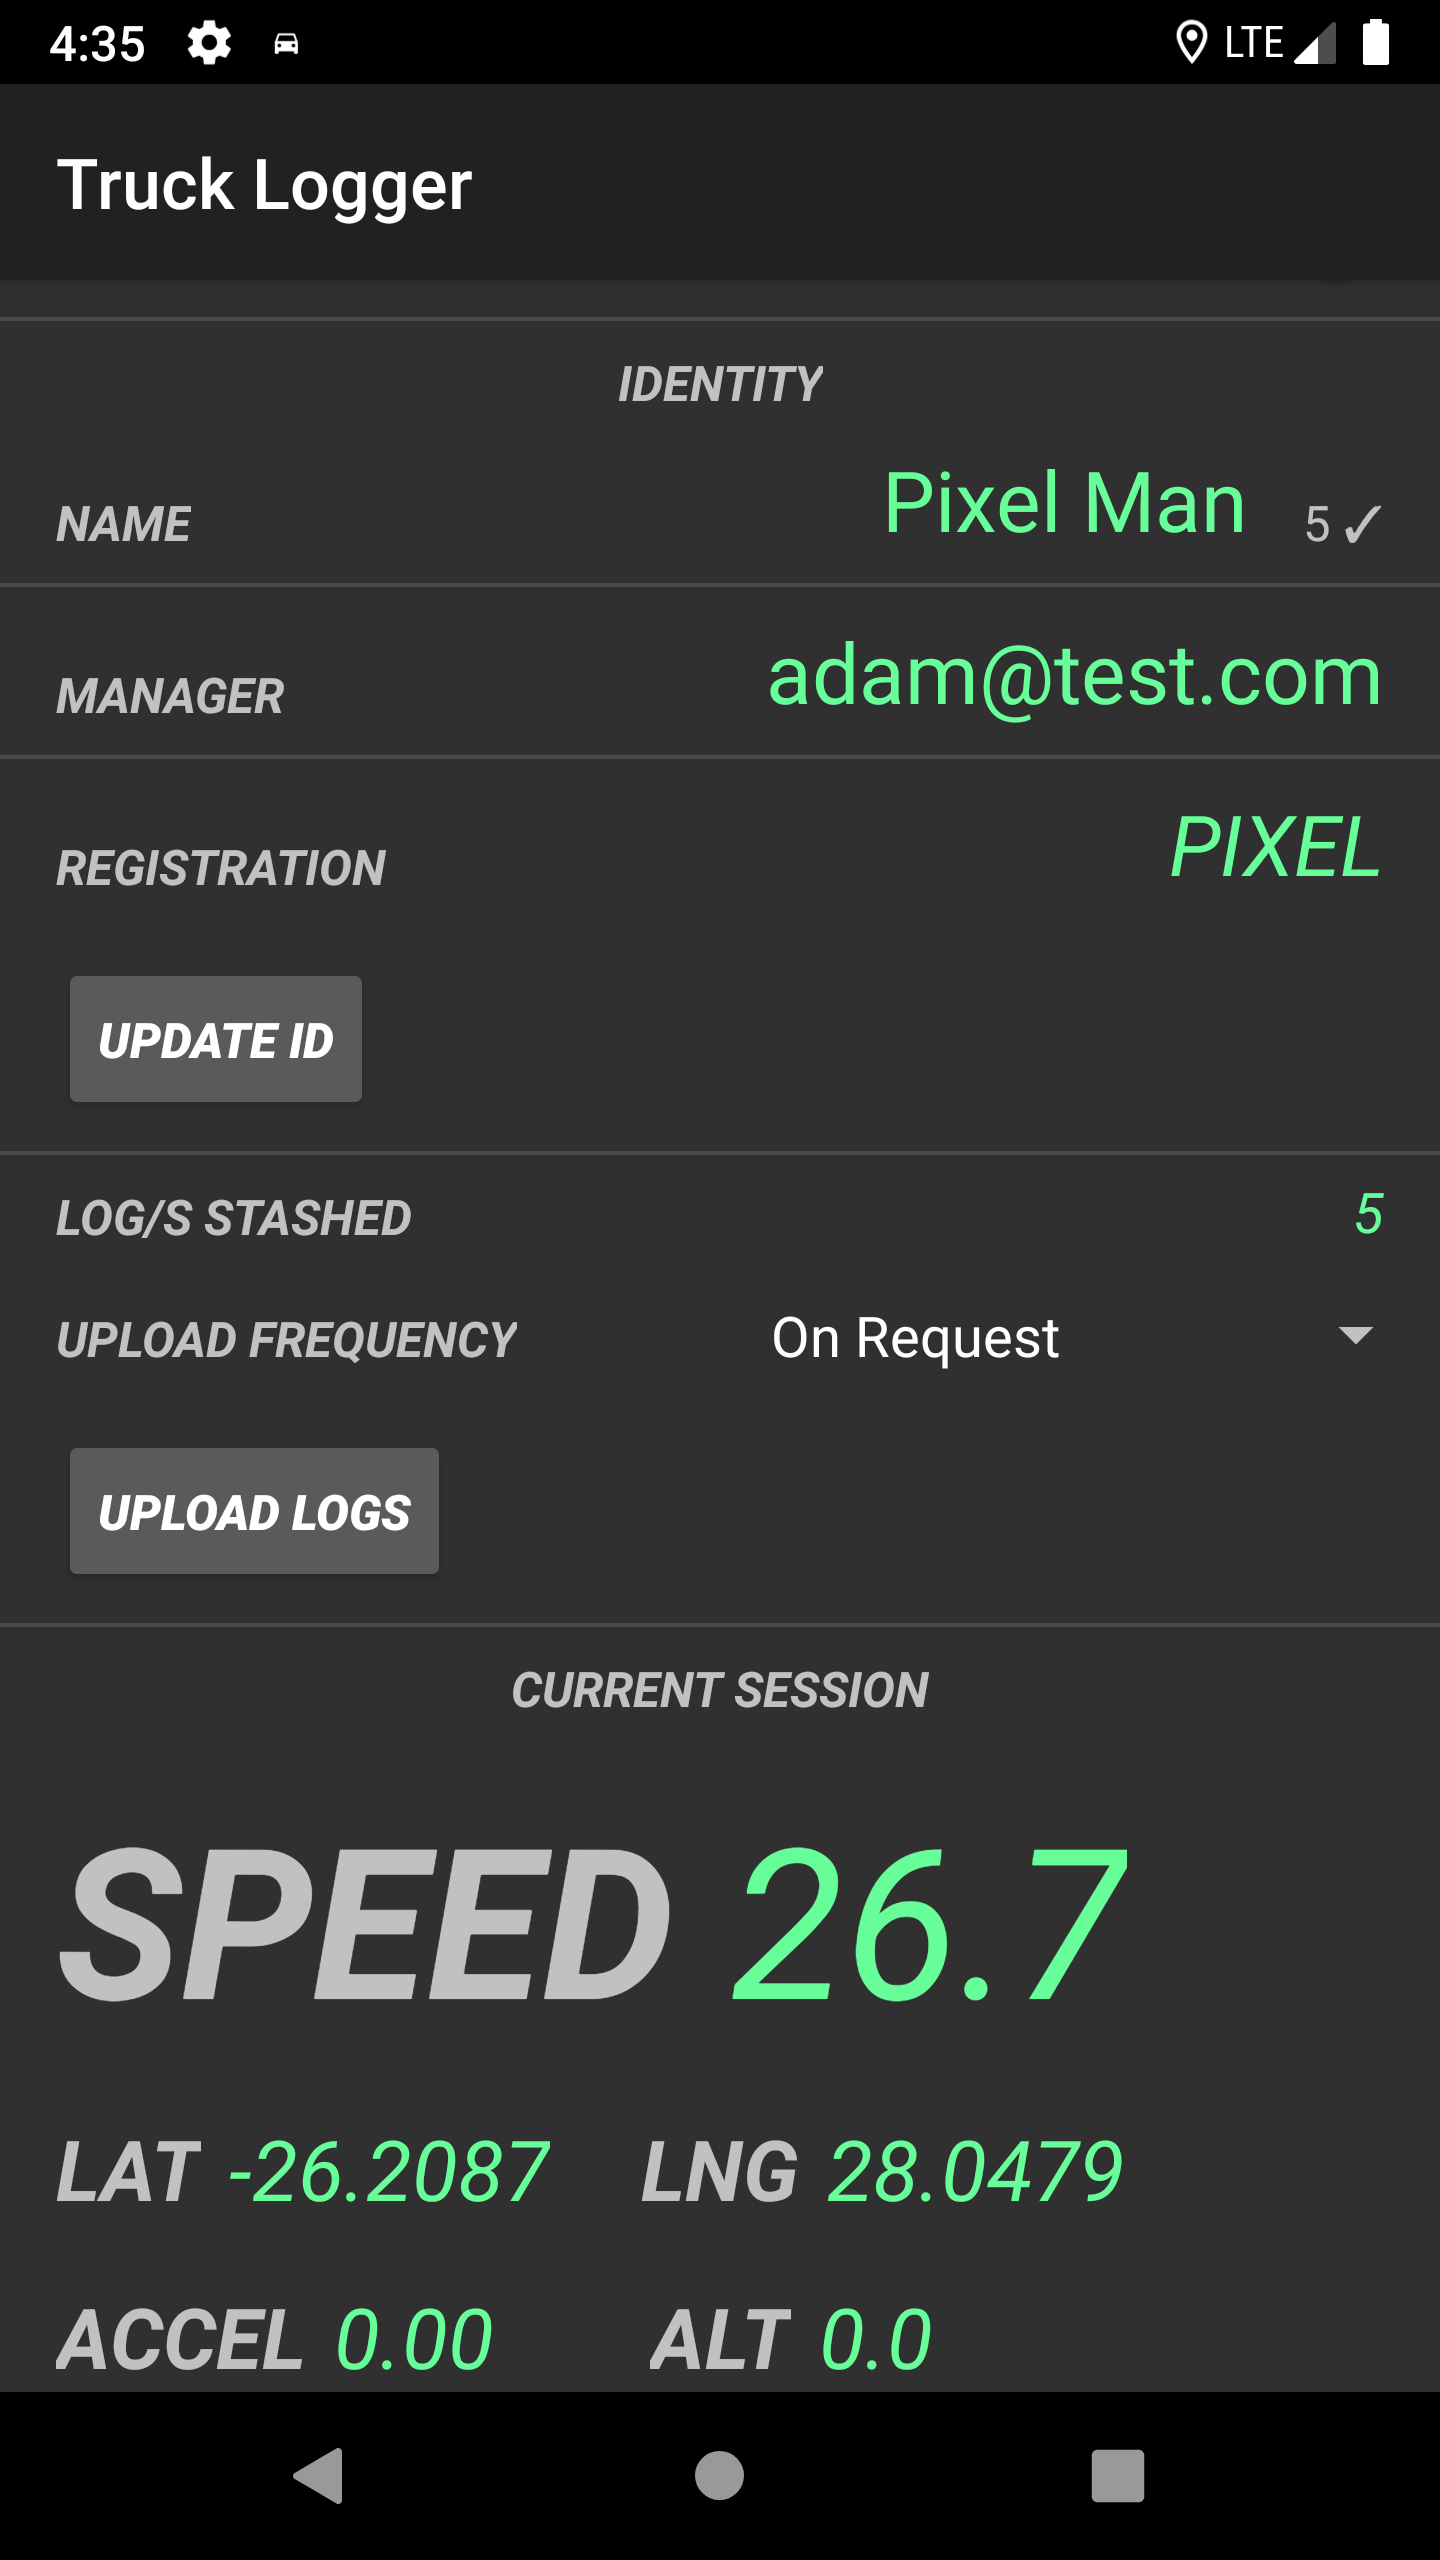
\includegraphics[height=2.5in]{android_app_stashing.png}
        \label{fig:android_app_stashing}
    }
\caption{Android application - Implemented layout}
\label{fig:android_app_implementation}
\end{figure}

The \ac{ui} provides an interface detailing \ac{id} information related to the trucker and manager.
Users can update their \ac{id} as long as they have connectivity to the server.
They can also upload all log data at any instance.

Figure \ref{fig:android_app_idle} depicts the application in an idle state.
The application performs no logging in this state.

Toggling the status check box allows the application to start logging data, as seen in figure \ref{fig:android_app_running}.
This activates the background process which polls for \ac{gps}, acceleration (provided the linear composite accelerometer if available) and altitude.
While tracking, a constant notification is displayed, indicating speed and number of logs stashed.

Depending on the upload frequency, an attempt is made to upload logs to the central server.
Otherwise logs are stashed in the SQLite database.

\subsection{\Ac{io} Server}
Figure \ref{fig:io_output} depicts the output of the \ac{io} server, logging request information to standard output.

\begin{figure}[H]
\centering
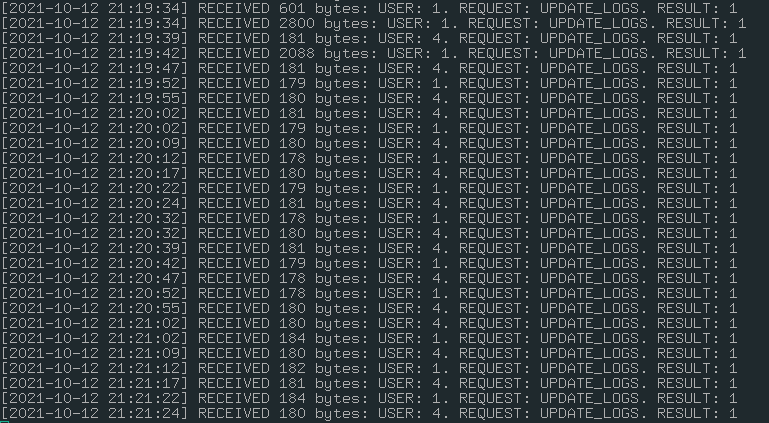
\includegraphics[scale=0.60]{io_output.png}
\caption{IO Server - Request information logged to standard output}
\label{fig:io_output}
\end{figure}

The \Ac{io} server handles \ac{ssl} connections transmitting a serialized \ac{json} payload consisting of the truckers \ac{id}, \ac{uuid} and extra data (detailed in figure \ref{fig:json_protocol}).
The \ac{uuid} is added to ensure that one trucker can be associated with a device.
Depending on the request code provided, the server processes each request appropriately.



\subsection{Web server}


\subsection{Deployment}

\pagebreak
